\documentclass[12pt]{article}
\usepackage[utf8]{inputenc}
\usepackage{geometry}
\geometry{a4paper, margin=1in}
\usepackage{amsmath}
\usepackage{amsfonts}
\usepackage{graphicx}
\usepackage{hyperref}
\usepackage{booktabs}
\usepackage{xcolor}
\usepackage{listings}

\hypersetup{
    colorlinks=true,
    linkcolor=blue,
    filecolor=magenta,      
    urlcolor=blue,
}

\title{ME 759 Intermediary Project Report\\ \Large FlashAttention in Raw CUDA}
\author{Gaurav Batra \\ \href{mailto:gbatra3@wisc.edu}{gbatra3@wisc.edu} \\ \textit{Computer Science (MS)}}
\date{\today}

\begin{document}

\maketitle

\vspace{-1.5em}
\begin{center}
    \textbf{Project Repository:} \url{https://github.com/batra98/me759-flashattention} \\
    \vspace{0.3em}
    \textbf{Interactive Educational Report:} \url{https://batra98.github.io/me759-flashattention}
\end{center}
\vspace{1em}

\begin{abstract}
Standard Transformer attention mechanisms suffer from $O(N^2)$ memory complexity. Calculating the dot product of every Query with every Key requires materializing a massive $N \times N$ matrix in High Bandwidth Memory (HBM). This intermediary report details the progress on developing a custom FlashAttention forward pass in bare-metal CUDA. By utilizing Shared Memory (SRAM) and reformulating the softmax computation, we successfully demonstrate a reduction in global memory traffic from $O(N^2)$ to $O(N)$, yielding a $1.8\times$ speedup and a $138\times$ reduction in memory writes at $N=4096$ on an NVIDIA Tesla T4. Furthermore, an interactive educational website has been built to visualize the Streaming Multiprocessor (SM) memory hierarchy.
\end{abstract}

\section{Introduction and Motivation}
In modern Deep Learning workloads, specifically autoregressive large language models, inference is fundamentally memory-bandwidth bound rather than compute-bound \cite{dao2022}. The standard attention formulation materializes the full $N \times N$ attention matrix $S$ in Global Memory (HBM). For sequence lengths like $N=4096$, writing this intermediate matrix to global memory, only to immediately read it back to compute the Softmax denominator, completely saturates the GPU memory bus.

While libraries like cuBLAS are highly optimized, they act as black boxes. Writing a custom FlashAttention kernel from scratch provides a deep understanding of hardware utilization. The objective of this project is to implement FlashAttention \cite{dao2022} completely from scratch in raw CUDA C++, benchmarking its latency and using NVIDIA Nsight Compute (NCU) to analytically verify the reduction in HBM traffic on an NVIDIA GPU.

\section{Methodology \& Algorithm Design}

\subsection{The Baseline (Naive) Implementation}
To form a solid experimental baseline, a standard three-kernel attention mechanism was implemented:
\begin{enumerate}
    \item \textbf{Score Kernel:} Computes $S = QK^T / \sqrt{d}$ and saves the full $N \times N$ matrix to HBM.
    \item \textbf{Softmax Kernel:} Loads rows from HBM, finds the moving maximum, exponentiates, and normalizes in a multi-pass approach over HBM lines.
    \item \textbf{Output Kernel:} Loads probabilities and $V$ from HBM, computing and writing the final output $O$ to HBM.
\end{enumerate}
This naive approach exhibits massive uncoalesced global reads and creates immense HBM thrashing.

\subsection{FlashAttention (Tiled, Shared Memory) Implementation}
To resolve the memory bottleneck, the algorithm was redesigned to leverage the 64 KB Shared memory (SRAM) available per SM on the Tesla T4 architecture. With chosen block sizes $B_r = 32$, $B_c = 32$, and $d = 64$, the required matrices fit comfortably into a 24 KB SRAM footprint.

\subsubsection{Online Softmax and Loop Tiling}
Instead of processing the entire $N \times N$ matrix at once, the $Q, K,$ and $V$ matrices are sliced into smaller blocks. We load a small block from global memory into SRAM and compute the attention scores. 

To prevent numerical overflow without requiring the entire row, we implement the Online Softmax algorithm \cite{milakov2018}. By maintaining a moving maximum ($m$) and a local normalization sum ($\ell$) directly within the ultra-fast thread registers, the denominator is updated incrementally:
\begin{equation}
m^{(j)}_i = \max\!\bigl(m^{(j-1)}_i,\; \tilde{m}_{ij}\bigr)
\end{equation}
\begin{equation}
\ell^{(j)}_i = e^{m^{(j-1)}_i - m^{(j)}_i}\,\ell^{(j-1)}_i + e^{\tilde{m}_{ij} - m^{(j)}_i}\,\tilde{\ell}_{ij}
\end{equation}
This allows the kernel to fuse the operations. The $O(N^2)$ logits are never written to HBM, as shown in this core CUDA block:

\begin{lstlisting}[language=C++, basicstyle=\ttfamily\footnotesize, frame=single, commentstyle=\color{green!60!black}]
// Online rescale: completely eliminating global memory writes
float m_new = fmaxf(m_i, m_tilde);
float alpha = expf(m_i - m_new);
float beta  = expf(m_tilde - m_new);

for (int k = 0; k < d; ++k) {
    float pv_k = 0.0f;
    for (int jj = 0; jj < bc_actual; ++jj)
        pv_k += S_row[jj] * V_smem[jj][k];
    O_acc[k] = alpha * O_acc[k] + beta * pv_k;
}
m_i = m_new;
l_i = alpha * l_i + beta * l_tilde;
\end{lstlisting}

\section{Experimental Setup}
\begin{itemize}
    \item \textbf{Hardware:} NVIDIA Tesla T4 (sm\_75, Turing Architecture, 8.1 TFLOPs FP32).
    \item \textbf{Compilation:} Compiled using \texttt{nvcc} via CMake with \texttt{-O3 --extended-lambda --expt-relaxed-constexpr -lineinfo}.
    \item \textbf{Validation:} Root Mean Square Error (RMSE) validation ensures discrepancy $< 10^{-3}$ against the naive baseline.
    \item \textbf{Measurement Tooling:} \texttt{cudaEvent} for latency, and \texttt{ncu} (NVIDIA Nsight Compute) for L1TEX bytes traffic evaluation.
\end{itemize}

\section{Results \& Benchmarks}

\subsection{Execution Latency (Speedup)}
FlashAttention exhibits steady and significant speedups. At $N=4096$, latency improved from $\approx 27.12$ ms to $\approx 14.96$ ms, yielding a \textbf{1.8$\times$ speedup}. At $N=8192$, latency improved from $\approx 112.31$ ms to $\approx 58.70$ ms. The latency is completely unblocked from the memory wall.

\begin{figure}[htbp]
    \centering
    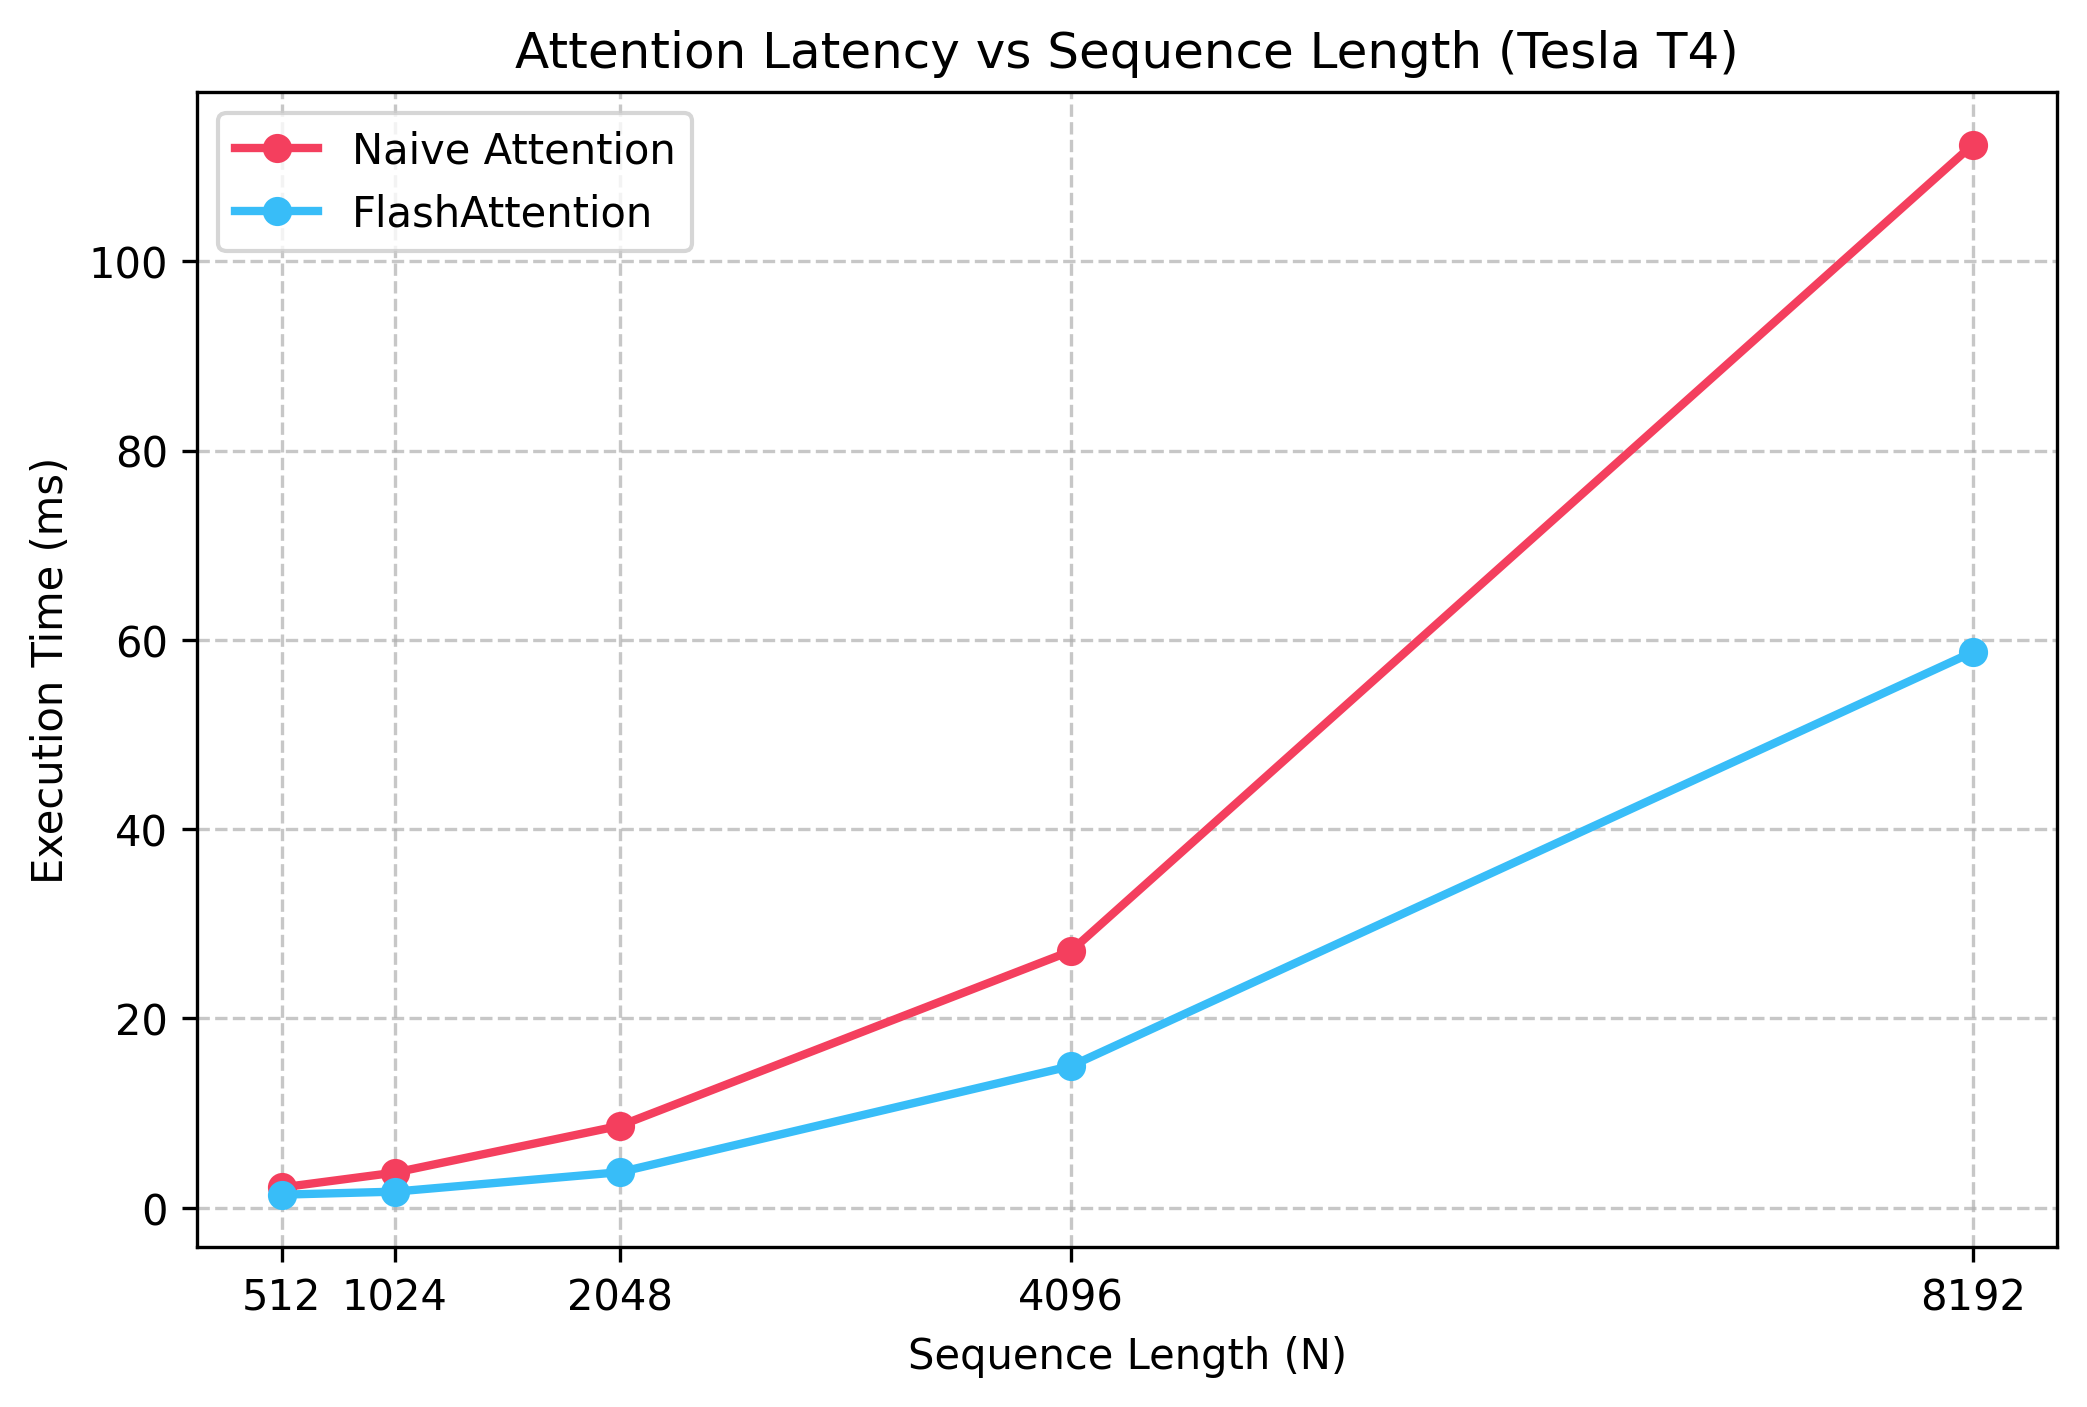
\includegraphics[width=0.75\textwidth]{docs/assets/latency_plot.png}
    \caption{Execution Latency vs Sequence Length.}
    \label{fig:latency}
\end{figure}

\subsection{HBM Traffic Reduction}
Nsight Compute telemetry confirms the core hypothesis. For $N=4096$:
\begin{itemize}
    \item \textbf{Naive Traffic:} $\approx 25.8$ GB read, $\approx 1.16$ GB write.
    \item \textbf{Flash Traffic:} $\approx 2.21$ GB read, $\approx 8$ MB write.
\end{itemize}
This represents an \textbf{$\approx 11\times$ reduction in reads} and an \textbf{$\approx 138\times$ reduction in writes}.

\begin{figure}[htbp]
    \centering
    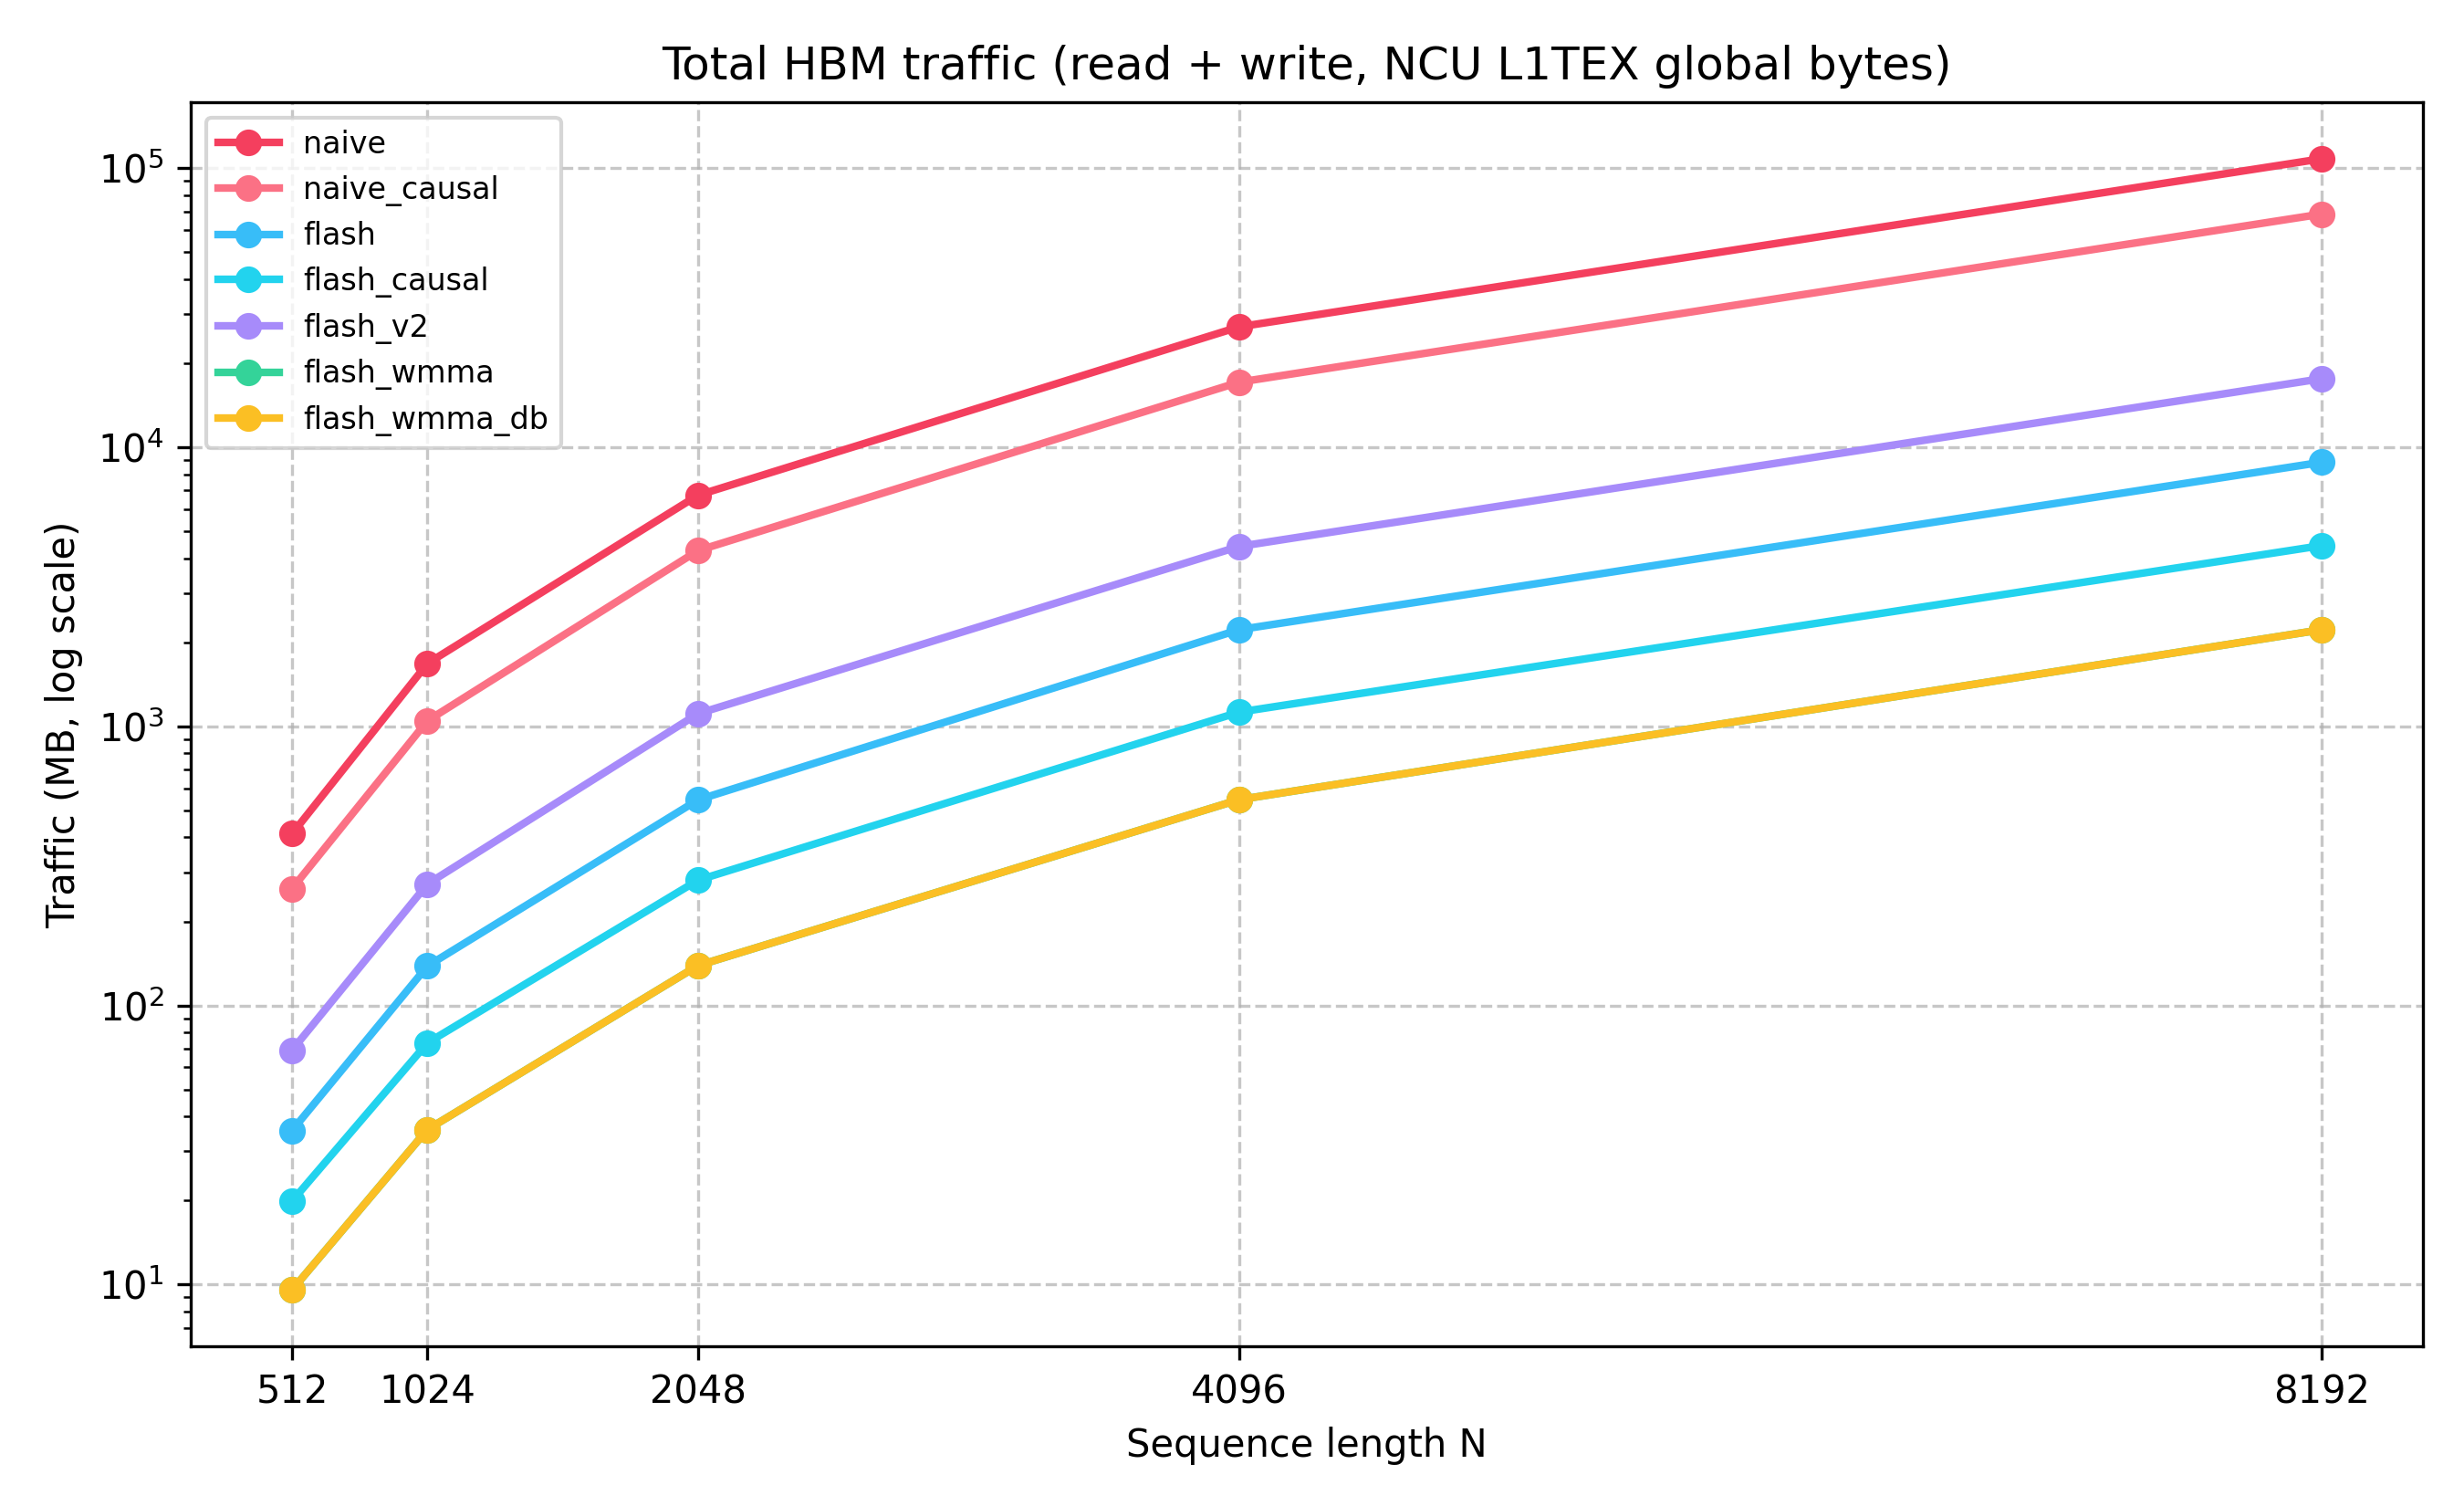
\includegraphics[width=0.75\textwidth]{docs/assets/hbm_plot.png}
    \caption{HBM Global Memory Traffic vs Sequence Length. Notice the quadratic scaling of the naive implementation.}
    \label{fig:hbm}
\end{figure}

\section{Interactive Educational Website}
Alongside the CUDA implementation, the project documentation has been transformed into a highly-readable technical blog hosted at \url{https://batra98.github.io/me759-flashattention}. 

A dynamic, CSS-driven state machine visually simulates a single Streaming Multiprocessor, including a glowing Data Bus, Global Memory blocks, SRAM tiles, and a pulsing 32-thread Warp Grid. This provides users with a direct visual intuition of the $O(N^2)$ HBM bottleneck versus SRAM data locality.

\section{Future Work \& Final Project Trajectory}
The current implementation successfully validates the FlashAttention logic in raw CUDA, achieving the theoretical $O(N)$ memory reduction. To construct the final comprehensive deliverable for ME 759, the project will implement the following advanced HPC optimizations to push the arithmetic intensity to the absolute hardware limits:

\subsection{Hardware Tensor Cores (WMMA)}
The current kernel utilizes standard FP32 execution units. The Tesla T4 Turing architecture features specialized Tensor Cores capable of executing mixed-precision Matrix-Multiply-Accumulate (MMA) operations incredibly fast. Future work will involve upgrading the inner dot-product computations to FP16 using the \texttt{nvcuda::wmma} API \cite{nvidia_wmma}, mapping the block-level math natively onto Tensor Cores.

\subsection{Double Buffering and \texttt{cp.async}}
Currently, the SM stalls while waiting for $K$ and $V$ tiles to load from HBM into Shared Memory. To maximize instruction throughput, the final kernel will implement hardware asynchronous memory copying (\texttt{cp.async}). By allocating a double-buffer in SRAM, the GPU can fetch the $(j+1)$-th tile from global memory concurrently while the compute cores process the $j$-th tile.

\subsection{Causal Masking Integration}
Autoregressive models (like GPT) only attend to past tokens, enforcing a lower-triangular causal mask on the $S$ matrix. Engineering the thread block logic to dynamically skip fetching and computing tiles that fall outside this causal mask will effectively halve the total FLOPs required.

\subsection{Warp-Level Primitives}
The Online Softmax implementation currently relies on block-level shared memory reductions. To eliminate the high overhead of \texttt{\_\_syncthreads()} barriers, the final architecture will replace these reductions with warp-synchronous \texttt{\_\_shfl\_down\_sync} primitives, enabling independent 32-thread warps to resolve their maximums entirely within the register file.

\subsection{Multi-GPU Distributed Attention (NCCL / MPI)}
To scale beyond a single Tesla T4, the project will investigate distributing the attention mechanism across multiple GPUs. By partitioning the Query matrix $Q$ across different GPU instances and communicating the required $K$ and $V$ blocks via NVIDIA Collective Communications Library (NCCL) or MPI protocols, the architecture can support massive sequence lengths that exceed the 16 GB capacity of a single GPU.

\begin{thebibliography}{9}

\bibitem{dao2022}
Dao, T., Fu, D. Y., Ermon, S., Rudra, A., \& Ré, C. (2022). 
\textit{FlashAttention: Fast and Memory-Efficient Exact Attention with IO-Awareness.} 
NeurIPS 2022. \url{https://arxiv.org/abs/2205.14135}

\bibitem{vaswani2017}
Vaswani, A. et al. (2017). 
\textit{Attention Is All You Need.} 
NeurIPS 2017. \url{https://arxiv.org/abs/1706.03762}

\bibitem{milakov2018}
Milakov, M. \& Gimelshein, N. (2018). 
\textit{Online normalizer calculation for softmax.} 
arXiv preprint. \url{https://arxiv.org/abs/1805.02867}

\bibitem{nvidia_wmma}
NVIDIA. 
\textit{CUDA C++ Programming Guide: Warp Matrix Functions (WMMA).} 
\url{https://docs.nvidia.com/cuda/cuda-c-programming-guide/index.html#warp-matrix-functions}

\end{thebibliography}

\end{document}
